% SPDX-FileCopyrightText: Copyright (c) 2023 Yegor Bugayenko
% SPDX-License-Identifier: MIT

\documentclass{article}
\usepackage{../../lecture-notes/notes}
\usepackage[russian,english]{babel}
\usepackage{svg}
\usepackage{bibentry}
\usepackage{fancyvrb}
\usepackage{tikz}
  \usetikzlibrary{shadows}

\graphicspath{{../../faces/}}

\newcommand*{\thetitle}{Rise and Fall of OOP}
\newcommand*{\thesubtitle}{{\selectlanguage{russian}Каковы перспективы?}}
\newcommand*{\theauthor}{Yegor Bugayenko}
\newcommand\hlt[1]{\textcolor{orange}{#1}}

\newenvironment{xcode}[1][xcode.txt]
  {\VerbatimEnvironment\begin{VerbatimOut}{#1}}
  {\end{VerbatimOut}}

\begin{document}

\pptLeft{%
  \includesvg[height=2em]{../../lecture-notes/logos/ngu.svg}\\
  April 11th, 2025}
\pptRight{@yegor256}

\lnPitch{
  \begin{pptMiddle}
    \includesvg[height=4em]{../../lecture-notes/logos/ngu.svg}
    \pptTitle{\thetitle}{\thesubtitle}\par
    {\scshape \theauthor}
    \newline
    {\small Huawei\par}
  \end{pptMiddle}
}
\newpage
\pagecolor{white}

% \pptToc

\lnPitch{
  \pptBanner{Why Me?}
  \begin{enumerate}
  \item \href{https://www.yegor256.com/elegant-objects.html}{\textbf{Elegant Objects}} books: No.1 in \href{https://www.goodreads.com/shelf/show/object-oriented-programming}{Goodreads} OOP shelf
  \item \href{https://www.eolang.org}{\textbf{EOLANG}}, pure object-oriented language: 1.2K\(\star\)
  % \item \(\varphi\)-calculus, object modeling formalism
  \item \href{https://www.takes.org}{\textbf{Takes}}, Java Web Framework: 800\(\star\)
  \end{enumerate}}

\lnPitch{\pptChapter[Intent]{Objects Are Abstractions}}

\lnPitch{
  \pptSection[SIMULA]{Why Did They Invent OOP?}
  \begin{multicols}{2}
  \pptPic{.95}{../../painofoop/01-algorithms/dahl-and-nygaard.jpg}\\
  \par\columnbreak\par
  SIMULA was created in 1965 at the Norwegian Computing Center in Oslo by Ole-Johan Dahl and Kristen Nygaard \hlt{to simulate} real-world systems. In doing so, it introduced core concepts of object-oriented programming, including objects, classes, inheritance, and virtual methods.
  \end{multicols}}

\lnPitch{
  \pptSection[Proxies]{Objects Are Proxies for Real Things}
  \begin{multicols}{2}
  \includegraphics[width=.95\linewidth]{../../painofoop/01-algorithms/abstraction.png}
  \par\columnbreak\par
  ``Object-oriented design is first concerned with \hlt{entities}---things. These things may be tangible objects such as traffic lights, chairs, or airplanes. From a design perspective, objects \hlt{model} the entities in the application domain.''
  \lnSource{korson1990understanding}
  \end{multicols}}

\lnQuote
  [Hemant Pande]
  {hemant-pande}
  {Dynamic binding and polymorphism, which only exist in objects, support \hlt{abstraction} and differentiate object-orientation from the \hlt{imperative} programming paradigm.}
  {pande1996data}

\begin{xcode}[animals.java]
interface Fruit
  void calories();
class Plum
  @Override
  void calories() { ... }
class Apple
  @Override
  void calories() { ... }

void cook(Fruit a)
  var c = a(*@\textcolor{orange}{.calories}@*)();
\end{xcode}
\lnPitch{
  \pptSection[Dynamic Dispatch]{1.~Dynamic Dispatch}
  \begin{multicols}{2}
  {\small\ffinput{animals.java}}
  \par\columnbreak\par
  ``The most important language feature that supports abstraction is the \hlt{dynamic dispatch} of methods based on the run-time type of an object.''
  \lnSource{bacon1996fast}
  \end{multicols}}

\lnPitch{
  \pptSection[Encapsulation]{2.~Encapsulation}
  \begin{multicols}{2}
  \includegraphics[height=1.5in]{../../painofoop/01-algorithms/apple.jpg}
  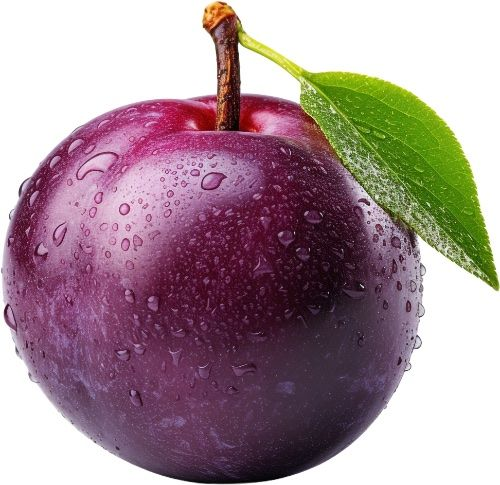
\includegraphics[height=1.2in]{plum.jpg}
  \begin{enumerate}
  \setlength\itemsep{0em}
  \item Weight: 120g
  \item Calories: 94.6
  \item Price: \$0.99
  \end{enumerate}
  \par\columnbreak\par
  ``Once an implementation is selected, it should be treated as a \hlt{secret} of the abstraction and hidden from most clients.''
  \lnSource{booch1994object}
  \end{multicols}}

\lnPitch{\pptChapter[Slow]{However, OOP Is Slow}}

\lnQuote
  [Craig Chambers]
  {craig-chambers}
  {OO languages contain a number of features that make programs \hlt{easier to write} but \hlt{slower to run}. Pure OO languages use message passing for all computation, avoiding built-in operators and control structures. All computation, even low-level operations like variable accessing, arithmetic, and array indexing, is performed by \hlt{sending messages} to objects.}
  {chambers1991making}

\lnQuote
  [Jeff Piper]
  {jeff-piper}
  {We observe that there is a substantial cost associated with a \hlt{full object-oriented design} in scientific programs, and that the current compilers and VMs have a room for substantial improvements in this area.}
  {budimlic1999cost}
\lnPitch{
  \pptSection[1.2]{JDK 1.2 Was Very Slow}
  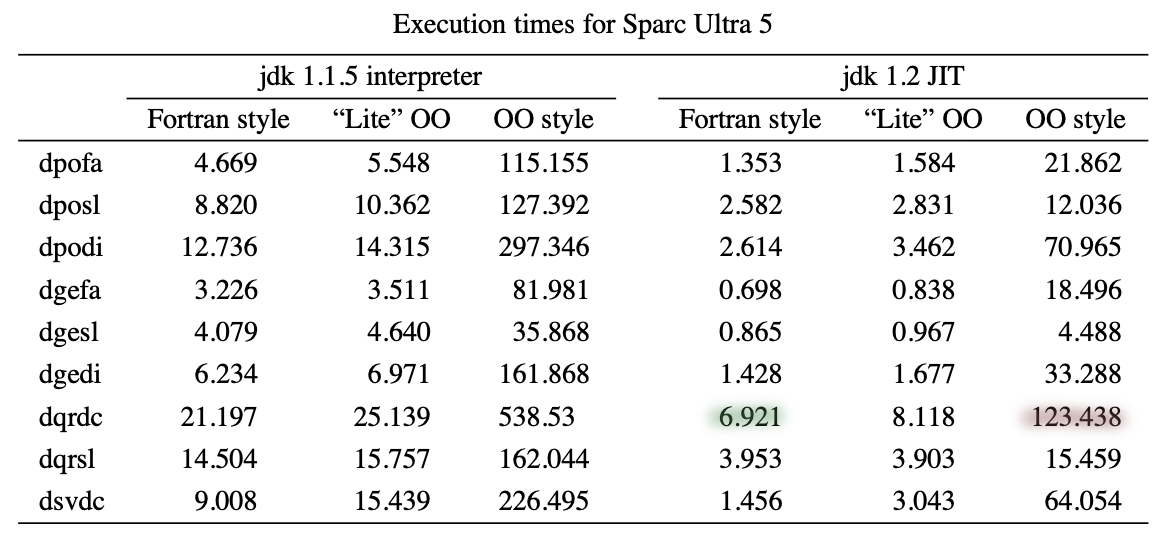
\includegraphics[width=.8\linewidth]{bulimic.png}\par
  \lnSource{budimlic1999cost}}
\lnPitch{
  \pptSection[23]{JDK 23 Is not Much Better}
  {\small\begin{tabularx}{\linewidth}{lX>{\ttfamily}r>{\ttfamily}r>{\ttfamily\arraybackslash}r}
  \toprule
  & & \multicolumn{2}{c}{CPU mInstructions} & \\
  Language & Compiler & {\rmfamily w/functions} & {\rmfamily w/objects} & {\rmfamily Ratio} \\
  \midrule
  C++ & clang 18.1.3 & 93 & 7,203 & \textcolor{orange}{76x} \\
  Java & javac 21.0.4 & 41 & 4,589 & \textcolor{orange}{109x} \\
  C\# & 8.0.108 & 36 & 5,785 & \textcolor{orange}{157x} \\
  Go & go1.22.2 & 39 & 15,907 & \textcolor{orange}{403x} \\
  Pascal & 3.2.2 & 59 & 32,804 & \textcolor{orange}{555x} \\
  \bottomrule
  \end{tabularx}}\par
  {\scriptsize The same Fibonacci algorithm was implemented in different programming languages using either functions (the third column) or objects (the forth column). Performance data was collected using \ff{perf} Linux tool (Ubuntu 20.04 at Intel Core i7, 16Gb, 3.3GHz), as millions of CPU instructions per a calculation of the 32\(^\text{nd}\) Fibonacci number. Source: \url{https://github.com/yegor256/fibonacci}.\par}}

\lnPitch{\pptChapter[Reasons]{Objects Are Slow for Two Reasons}}

\lnQuote
  [Bruno Dufour]
  {bruno-dufour}
  {\hlt{Virtual method dispatching} and \hlt{on-heap allocating} are the two primary sources of performance inefficiencies in object-oriented programs.}
  {dufour2003dynamic}

\begin{xcode}[streams.java]
var acc = Stream.of(VALUES)
  .map(obj -> (String) obj)
  .map(String::trim)
  .filter(str -> str.length() == 4)
  .map(str -> Long.parseLong(str, 16))
  .mapToLong(num -> num)
  .sum();
\end{xcode}
\begin{xcode}[loop.java]
var acc = 0L;
for (int i = 0; i < VALUES.length; i++) {
  var s = ((String) VALUES[i]).trim();
  if (s.length() != 4) continue;
  acc += Long.parseLong(s, 16);
}
\end{xcode}
\lnPitch{
  \pptSection[Streams]{For Example, Java Stream API vs. Loop}
  \begin{multicols}{2}
  Calculating the sum with the help of Stream API with OpenJDK Zulu~23.30:
  \par\columnbreak\par
  Exactly the same algorithm, but in imperative procedural style:
  \end{multicols}
  \par
  \begin{multicols}{2}
  {\scriptsize\ffinput{streams.java}\par}
  \par\columnbreak\par
  {\scriptsize\ffinput{loop.java}\par}
  \end{multicols}
  \par
  \begin{multicols}{2}
  \textcolor{red}{\textbf{154}} milliseconds.
  \par\columnbreak\par
  \textcolor{green}{\textbf{26}} milliseconds.
  \end{multicols}
  {\scriptsize The \ff{VALUES} contains 10 million strings, on MacBook M2~Pro 3.5~GHz.\par}}

\lnPitch{\pptChapter[Compilers]{Compilers May Help}}

\lnQuote
  [Zoran Budimli{\'c},]
  {zoran-budimlic}
  {Although Java implementations have been made great strides, they still fall short on programs that use the full power of Java’s object-oriented features. Ideally, future compiler technologies will be able to \hlt{automatically transform} the [OO style code] into something that approaches the [procedural style] in performance.}
  {budimlic1999cost}

\lnPitch{\pptChapter[ALGOL]{Instead: ALGOL in Java Syntax}}

\begin{xcode}[static.java]
var bytes = "Hello".getBytes();
Files.(*@\textcolor{orange}{write}@*)(path, bytes);
\end{xcode}
\begin{xcode}[no-static.java]
"Hello".toBytes().(*@\textcolor{orange}{saveTo}@*)(path);
\end{xcode}
\lnPitch{
  \pptSection[Static]{Issue \#1: Egocentric Static Methods}
  \begin{multicols}{2}
  In Java, we do this:
  {\small\ffinput{static.java}\par}
  Instead of this:
  {\small\ffinput{no-static.java}\par}
  \par\columnbreak\par
  ``Data manipulated and moved by active procedures are passive and helpless. Procedures tend to be \hlt{egocentric} and think that all data, its definitions and its values, are properly determined by the procedure currently using that data. The result is data that is \hlt{inconsistent} in definition and value.''
  \lnSource{west2004object}
  \end{multicols}}

\begin{xcode}[with-null.java]
var u = getUser(42);
(*@\textcolor{orange}{if (u == null)}@*)
  return "Not found";
var n = u.getName();
\end{xcode}
\begin{xcode}[without-null.java]
var n = user(42).(*@\textcolor{orange}{name}@*)();
\end{xcode}
\lnPitch{
  \pptSection[NULL]{Issue \#2: NULL, the Billion Dollar Mistake}
  \begin{multicols}{2}
  We do this:
  {\small\ffinput{with-null.java}\par}
  Instead of this:
  {\small\ffinput{without-null.java}\par}
  \par\columnbreak\par
  ``This led me to suggest that the null value is a member of every type, and a \hlt{null check is required} on every use of that reference variable, and it may be perhaps a billion dollar mistake.''
  \lnSource{hoare2009null}
  \end{multicols}}

\begin{xcode}[inheritance.java]
class Book (*@\textcolor{orange}{extends File}@*)
  void title()
    var t = (*@\textcolor{orange}{this.}@*)read();
    return t.find("title");
\end{xcode}
\begin{xcode}[composition.java]
class Book
  (*@\textcolor{orange}{File file;}@*)
  void title()
    var t = (*@\textcolor{orange}{file.}@*)read();
    return t.find("title");
\end{xcode}
\lnPitch{
  \pptSection[Inheritance]{Issue \#3: Implementation Inheritance}
  \begin{multicols}{2}
  We do this:
  {\small\ffinput{inheritance.java}\par}
  Instead of this:
  {\small\ffinput{composition.java}\par}
  \par\columnbreak\par
  ``Favoring object composition over class inheritance helps you keep each class encapsulated and focused on one task. Your classes and class hierarchies will remain small and will be less likely to grow into \hlt{unmanageable monsters}.''
  \lnSource{gamma1994design}
  \end{multicols}}

\begin{xcode}[mutable.java]
var c = new Circle();
c.setRadius(42.0);
c.setColor("blue");
\end{xcode}
\begin{xcode}[immutable.java]
var c = new Circle()
  .resize(42.0)
  .repaint("blue");
\end{xcode}
\lnPitch{
  \pptSection[Mutability]{Issue \#4: Mutable State}
  \begin{multicols}{2}
  We do this:
  {\small\ffinput{mutable.java}\par}
  Instead of this:
  {\small\ffinput{immutable.java}\par}
  \par\columnbreak\par
  ``Immutable classes are \hlt{easier to design}, implement, and use than mutable classes. They are less prone to error and are more secure.''
  \lnSource{bloch2008effective}
  \end{multicols}}

\lnQuote
  [David West]
  {david-west}
  {The contemporary mainstream understanding of objects (which is \hlt{not behavioral}) is but a pale shadow of the original idea and anti-ethical to the original intent.}
  {west2004object}

\lnPitch{\pptChapter[Disaster]{OOP Is a Disaster}}

\lnQuote
  [Alan Kay]
  {alan-kay}
  {I made up the term `object-oriented,' and I can tell you I didn't have C++ in mind.}
  {kay97keynote}

\lnQuote
  [Edsger Dijkstra]
  {edsger-dijkstra}
  {Object oriented programs are offered as alternatives to correct ones... Object-oriented programming is an \hlt{exceptionally bad idea} which could only have originated in California.}
  {crawford1989}

\lnQuote
  [Linus Torvalds]
  {linus-torvalds}
  {C++ is a \hlt{horrible language}$\dots$ C++ leads to really, really bad design choices$\dots$ In other words, the only way to do good, efficient, and system-level and portable C++ ends up to limit yourself to all the things that are basically available in C.}
  {schindler2007}

\lnQuote
  [Jeff Atwood]
  {jeff-atwood}
  {OO seems to bring at least as \hlt{many problems} to the table as it solves.}
  {atwood2007}

\lnQuote
  [Rich Hickey]
  {rich-hickey}
  {I think that large objected-oriented programs struggle with increasing complexity as you build this large object graph of \hlt{mutable objects}. You know, trying to understand and keep in your mind what will happen when you call a method and what will the side effects be.}
  {hickey2010}

\lnPitch{\pptChapter[Pure]{Let's Make OOP Great Again}}

\lnPitch{
  \pptBanner{``Pure'' Objects Are Possible:}
  \begin{itemize}
  \setlength\itemsep{0em}
  \item No static methods or attributes
  \item No mutability of state
  \item No implementation inheritance
  \item No NULL references
  \item No reflection, no annotations, no classes
  \end{itemize}
  In some languages most objects are pure,
  for example in \hlt{Self}, \hlt{Io}, and \hlt{EO}.}

\lnPitch{\pptChapter[Fast]{Can We Make Them Fast?}}

\lnThought{We can design a strict and ``pure'' language, without procedures, NULL references, and mutability.}

\lnThought{Because objects are less complex, in compile time, we can inline them, turning into procedures.}

\lnThought{We can place more objects on stack.}

\lnThought{We can create hardware with object-oriented instruction set that would include NEW and CALL directives.}

\lnPitch{
  \begin{multicols}{2}
  \pptBanner{1.~Subscribe:}\par
  \qrcode[height=8em]{https://t.me/yegor256news}\par
  \href{https://t.me/yegor256news}{\texttt{@yegor256news}}
  \par\columnbreak\par
  \pptBanner{2.~Join:}\par
  Text me in Telegram, to join EOLANG research project:\par
  {\Huge\texttt{@yegor256}}
  \end{multicols}}

\end{document}
